\section{Two-phase consolidation}

For the two-phase system the governing equations presented in the previous sections must be expanded slightly.

\subsubsection*{Fluid mass and momentum balance}
Following the same mass balance procedure as for the single phase case, and gathering two mass balance equations, one for a wetting fluid (i.e. liquid) and one for a non-wetting (i.e. gas) fluid, we write,

\begin{equation}
\begin{split}
{{S}_{w}}\left( \frac{\phi }{{{K}_{w}}}+\frac{\alpha -\phi }{{{K}_{s}}} \right)\frac{d{{p}_{w}}}{dt}-\phi \frac{d{{S}_{nw}}}{dt}+... \\
\nabla \cdot \left\{ \frac{\mathbf{k}k_{w}^{r}}{{{\mu }_{w}}}\left( -\nabla {{p}_{w}}+{{\rho }_{w}}\mathbf{g} \right) \right\}+\alpha {{\text{S}}_{w}}\nabla \cdot \frac{\partial \mathbf{u}}{\partial t}=0
\end{split}
\label{eq:H2liq}
\end{equation}

for mass balance of the wetting fluid, subscript $w$, and,

\begin{equation}
\begin{split}
{{S}_{nw}}\left( \frac{\phi }{{{K}_{nw}}}+\frac{\alpha -\phi }{{{K}_{s}}} \right)\frac{d{{p}_{w}}}{dt}+\phi \left( 1-\frac{{{S}_{nw}}}{{{K}_{nw}}}\frac{\partial {{p}_{c}}}{\partial {{S}_{w}}} \right)\frac{d{{S}_{nw}}}{dt}+... \\
\nabla \cdot \left\{ \frac{\mathbf{k}k_{nw}^{r}}{{{\mu }_{nw}}}\left( -\nabla {{p}_{w}}-\frac{\partial {{p}_{c}}}{\partial {{S}_{w}}}\nabla {{S}_{nw}}+{{\rho }_{nw}}\mathbf{g} \right) \right\}+\alpha {{S}_{nw}}\nabla \cdot \frac{\partial \mathbf{u}}{\partial t}= 0
\end{split}
\label{eq:H2gas}
\end{equation}

for mass balance of the non-wetting fluid, subscript $nw$. In these equations, $k^{r}_{\alpha }$ is relative permeability of phase $\alpha $, $\rho _{\alpha }$ is density of phase $\alpha $, and we have chosen wetting pressure, $p_w$, and non-wetting saturation, $S_{nw}$, as primary variables in the solution scheme. Other primary variables, such as capillary pressure, $p_c$, and non-wetting pressure, $p_{nw}$, could also have been chosen with algebraic manipulation, but our benchmark example requires constant, $p_c=0$, capillary pressure for comparison with an anylitical solution. This is not possible, of course, if $p_c$ is a primary variable. Any viable permeability saturation function may be chosen for the example, we use the Brooks-Corey function.

For the numerical solution, storage due to two different fluids with two different compressibilities and densities is handled implicitly with solution of the above equations. For the analytical solution, we must define an effective compressibility as a function of fluid saturation and properties of each fluid. For immiscible fluids without penetrating bubbles, two compressible materials behave as resistors in series with respect to bulk modulus, thus the effective modulus is

\begin{equation}
\frac{1}{{{K}_{f}}}=\frac{{{S}_{w}}}{{{K}_{w}}}+\frac{{{S}_{nw}}}{{{K}_{nw}}}.
\end{equation}

\subsubsection*{Solid momentum balance}

As with the single phase case, balance of linear momentum is defined by,

\begin{equation}
\frac{\partial {{\sigma }_{ij}}}{\partial {{x}_{j}}}+{{F}_{i}}=0,
\end{equation}

but now the body force is a function of two fluids, $F=\rho _m \text{g}$ for the mixture density $\rho _m =\phi (S_w \rho _w + S_{nw} \rho _{nw}) + (1-\phi )\rho _s$, and insertion of the elastic consitutive law yields for solid displacement,

\begin{equation}
\frac{\partial }{\partial {{x}_{j}}}\left[ G\frac{\partial {{u}_{i}}}{\partial {{x}_{j}}}+\left( \lambda +G \right)\frac{\partial {{u}_{j}}}{\partial {{x}_{i}}}-\alpha \bar{p}{{\delta }_{ij}} \right]+{{F}_{i}}=0,
\end{equation}

where \textit{mean} fluid pressure is defined as $\bar{p}=S_wp_w + S_{nw}p_{nw}$.

\subsubsection*{FEM solution scheme}
For the two-phase simulations, the two fluid balance equations are solved in a single global equation, with an iterative coupling to the solid balance equation. 

%-------------------------------------------------------------------------
%-------------------------------------------------------------------------

\subsection{Terzaghi consolidation: Two-phase}
\subsubsection*{Definition}
For this comparison, we may utilize the same analytical solution as was done for the single phase case in the previous section, although the solution must represent the mean fluid pressure $\bar{p}=S_wp_w + S_{nw}p_{nw}$, for the final relationship,

\begin{equation}
\frac{\bar{p}\left( z,t \right)}{\bar{p}_0}=\left\{ 1.0-{{\left( \frac{L-z}{L} \right)}^{2}}-\frac{32}{{{\pi }^{3}}}\left[ \sum\limits_{m=0}^{\infty }{\frac{{{\left( -1 \right)}^{m}}}{{{\left( 2m+1 \right)}^{3}}}\exp \left[ -{{\psi }^{2}}ct \right]\cos \left[ \psi \left( L-z \right) \right]} \right] \right\},
\end{equation} 

with pressure generation defined in the same manner,

\begin{equation}
{{\bar{p}}_{0}}=\frac{{{L}^{2}}}{2c}\left( {{B}_{v}}{{{\dot{\sigma }}}_{z}} \right),
\end{equation}

but where the uniaxial Skempton coefficient, ${B}_{v}$, must be defined (see Table \ref{terz:tab1}) based upon the effective fluid modulus. Fluid properties are then defined for two separate fluids (Table \ref{terz:tab4})

\begin{table}[!t]
\begin{center}
\begin{tabular}{lccc}
\hline\noalign{\smallskip}
Property & Symbol & Unit & Value \\
\noalign{\smallskip}\hline\noalign{\smallskip}
\textit{Wetting fluid properties} &          &        & \\
Bulk modulus   & $K_{w}$       & $GPa$       & $2.933$ \\
Density        & $\rho _{w} $  & $kg/m^3$    & $997.05$ \\
Viscosity      & $\mu _{w} $   & $Pa\dot s$  & $8.9008\times 10^{-4}$ \\
Saturation     & $S_{w}$       & $-$         & $0.8$ \\
\\
\textit{Non-wetting fluid properties} &               &               &  \\
Bulk modulus   & $K_{nw}$        & $GPa$       & $1.187$ \\
Density        & $\rho _{nw} $   & $kg/m^3$    & $997.05$ \\
Viscosity      & $\mu _{nw} $    & $Pa\dot s$  & $8.9008\times 10^{-4}$ \\
Saturation     & $S_{nw}$        & $-$         & $0.2$ \\
\noalign{\smallskip}\hline
\end{tabular}
\end{center}
\caption{Two-phase fluid properties.}
\label{terz:tab4}
\end{table}

\begin{figure}[!tbh]
\begin{center}
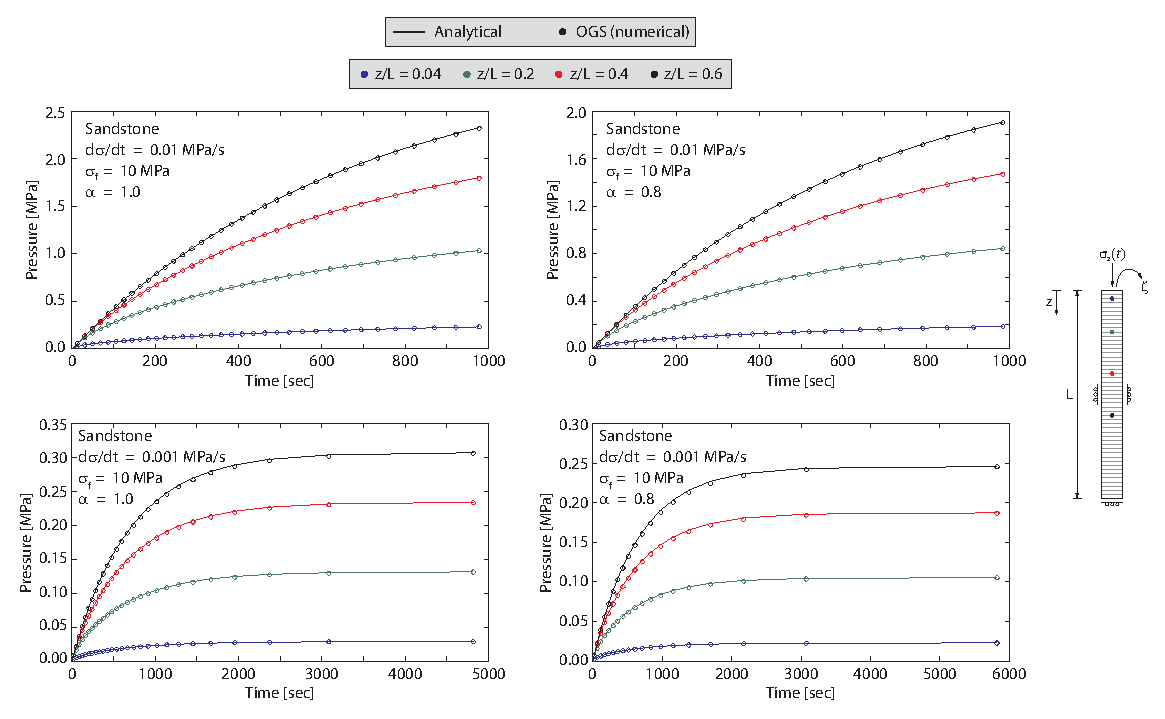
\includegraphics[width=1.0\textwidth]{chapter_14/figures/fig_14_3_21}
\end{center}
\caption{Sandstone solutions.}
\label{terz:h2msand}
%\end{figure}
%\begin{figure}[!tbh]
\begin{center}
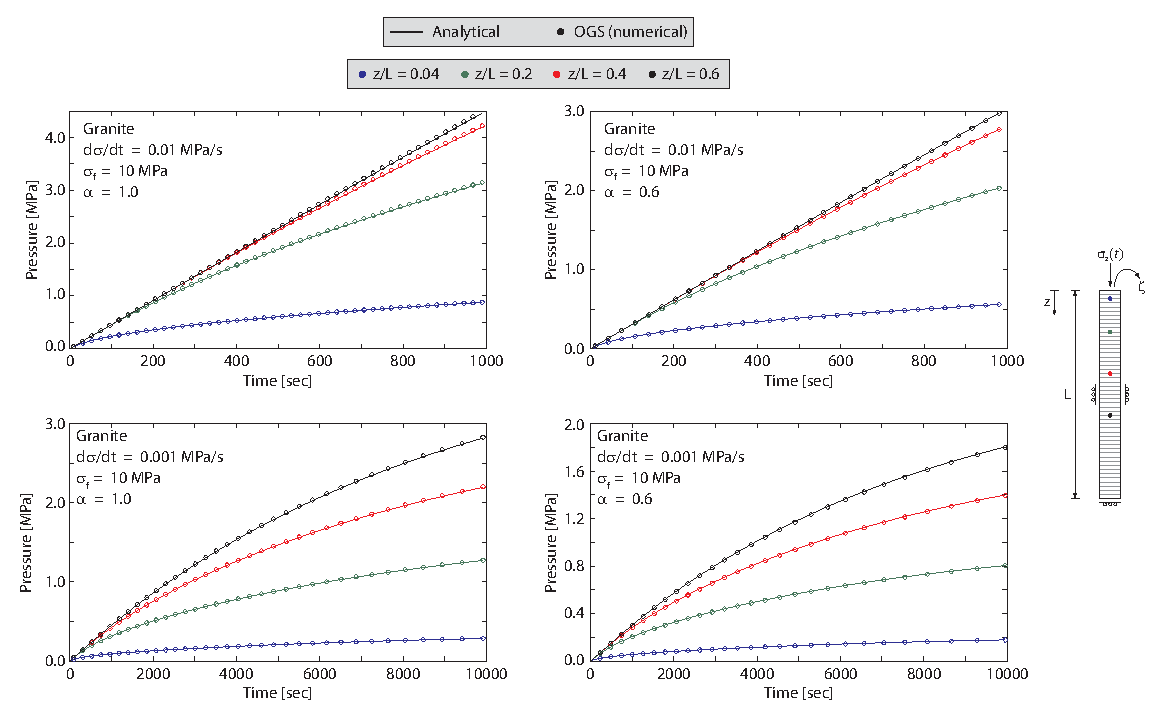
\includegraphics[width=1.0\textwidth]{chapter_14/figures/fig_14_3_22}
\end{center}
\caption{Granite solutions. Here, a porosity of 0.06 is used to ensure stability for the incompressible grain simulations (an adjustment that is not needed for compressible grains, but is used there also to maintain consistency).}
\label{terz:h2mgranite}
\end{figure}

\subsubsection*{Results}
Initially the column is at zero pressure and is saturated uniformly with both fluids ($Sw=0.8$) and we apply $p_c=0$ and $k^{r}_{w}=k^{r}_{nw}=0.5$. Note that we utilize a different compressibility for each fluid in order to exercise both fluid balance equations, with the analytical solution obtained using the \textit{effective} fluid modulus, and with the \textit{effective} modulus having an identical value to the single fluid modulus, $2.27 GPa$, used above in the single phase case.

Results are shown in Figs. \ref{terz:h2msand} and \ref{terz:h2mgranite} for sandstone and granite (see Table \ref{terz:tab2}) for incompressible and compressible grains. With reference to the staggered stability criterion discussed in the HM problem above, because we are examining incompressible grains here the solution becomes unstable for granite. Therefore, an alternate value of porosity (0.06) is utilized (in the granite simulations) to ensure stability, which results in $B_v<0.5$. Such an adjustment is not required when compressible (real) grains are used, but is utilized none-the-less for comparison with the incompressible grain solution. All results are ideally accurate. 

Time steps are adaptively controlled with a tolerance based on the rate of pressure change over a time step. Such a scheme is capable of ensuring accuracy in HM or H2M problems. Note the importance of the tolerance in Fig. \ref{terz:res1}.

\subsection{Invarient stress: Flow and storage in a compressible medium}

It is also possible, and sometimes useful, to test two-phase storage and pressure dissipation in a deformable media at invarient stress. This test guarantees accurate implementation of fluid storage within the mass matrix (time derivative term) of the fluid mass balance PDE. 

\subsubsection*{Definition}
We utilize the same problem as above, but now no stress is applied and no mechanical equilibrium performed. The analytical solution may be derived from the Carslaw and Jaeger \cite{Carslaw:59} solution for heat dissipation within a solid slab,

\begin{equation}
\bar{p}\left( z,t \right)=\frac{4{{p}_{0}}}{\pi }\sum\limits_{m=0}^{\infty }{\left\{ \frac{1}{2m+1}\sin \left[ z\left( \frac{\left( 2m+1 \right)\pi }{2L} \right) \right]\exp \left[ -ct{{\left( \frac{\left( 2m+1 \right)\pi }{2L} \right)}^{2}} \right] \right\}},
\end{equation}

where $\bar{p}_0$ is initial mean pressure within the column.

\begin{figure}[!b]
\begin{center}
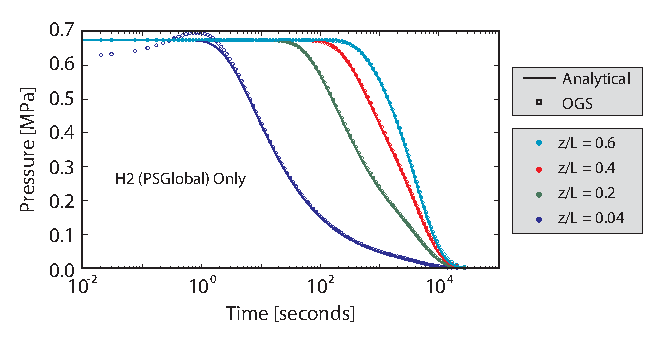
\includegraphics[width=0.7\textwidth]{chapter_14/figures/fig_14_3_23}
\end{center}
\caption{Two-phase flow with mechanical storage.}
\label{terz:h2}
\end{figure}

\subsubsection*{Results}
Results are shown in Fig. \ref{terz:h2}. We note that with an appropriate mixing rule for storage in the two phase formulation, the result is ideal.  Very small values of time and $z$ can produce inaccuracies; however, this will always be the case, barring a very small mesh discretization.
\subsection{Cam-Clay consolidation with swelling}
As before, equations \ref{eq:H2liq} and \ref{eq:H2gas} define the fluid system. In this example, however, we choose a numerical solution in OpenGeoSys that accomodates pressure variables in the solution vector. Both equations are therefore algebraically manipulated so that the primary variables to solve for are now the capillary pressure, $p_c$, and the non-wetting pressure, $p_{nw}$,

\begin{equation}
\phi {{\rho }_{w}}\frac{\partial {{S}_{w}}}{\partial {{p}_{c}}}\frac{d{{p}_{c}}}{dt}+{{\rho }_{w}}{{S}_{w}}\nabla \cdot \frac{d\mathbf{u}}{dt}+\nabla \cdot \left[ {{\rho }_{w}}\frac{\mathbf{k}k_{w}^{r}}{{{\mu }_{w}}}\left( -\nabla {{p}_{nw}}+\nabla {{p}_{c}}+{{\rho }_{w}}\mathbf{g} \right) \right]={{Q}_{w}}
\end{equation}

\begin{equation}
\begin{split}
%\begin{align}
  & -\phi {{\rho }_{nw}}\frac{\partial {{S}_{w}}}{\partial {{p}_{c}}}\frac{d{{p}_{c}}}{dt}+\phi \left( 1-{{S}_{w}} \right)\left( \frac{\partial {{\rho }_{nw}}}{\partial {{p}_{nw}}}\frac{d{{p}_{nw}}}{dt}+\frac{\partial {{\rho }_{nw}}}{\partial {{p}_{c}}}\frac{d{{p}_{c}}}{dt} \right)+ \\ 
 & \text{          }\left( {{\rho }_{w}}{{S}_{w}}+{{\rho }_{nw}}\left( 1-{{S}_{w}} \right) \right)\nabla \cdot \frac{d\mathbf{u}}{dt}+\nabla \cdot \left[ {{\rho }_{nw}}\frac{\mathbf{k}k_{nw}^{r}}{{{\mu }_{nw}}}\left( -\nabla {{p}_{nw}}+{{\rho }_{nw}}\mathbf{g} \right) \right]={{Q}_{nw}} \\ 
%\end{align}
\end{split}
\end{equation}

where in this case we assume that solid grains are incompressible. 

As in Section 14.2, swelling stress is based on the linear swelling model proposed by Rutqvist (2005) \cite{Jonny05}, which defines the increment of swelling stress to be proportional to liquid saturation increment,

\begin{equation}
\Delta \sigma ^{sw}=\beta \Delta S_w,
\end{equation}

where $\beta $ is a swelling coefficient that could be called the maximum swelling stress. As the saturation change approaches unity, swelling stress approaches $\beta $.

\subsubsection*{Definition}
Fig. \ref{fig_aximodel} shows the axi-symmetric model domain for the confined swelling test as well as the initial and boundary conditions for the two-phase flow consolidation problem with hydraulic and fluid properties are given in Table \ref{tab:hydromat}. The parameters of the elasto-plastic swelling model are given in Table \ref{tab:pls} for Cam-Clay plasticity.

\begin{figure}[!tbh]
\centering
\scalebox{0.5} % Change this value to rescale the drawing.
{
\begin{pspicture}(0,-8)(17.45797,8)
\psframe[linewidth=0.04,dimen=outer](10,7.5)(7,-7.5)
\usefont{T1}{ptm}{m}{n}
\rput(8.526719,0.1696875){
\begin{minipage}{0.12\textwidth}
{\color{blue}
\begin{align*}
&p^c=84.6\mbox{MPa}\\
&p^g=0.1\mbox{MPa}
\end{align*}
}
{\color{red}
\begin{align*}
&\sigma_x=0.1\mbox{MPa}\\
&\sigma_y=0.1\mbox{MPa}\\
&\sigma_z=0.1\mbox{MPa}\\
&\sigma_{xy}=0\\
&\sigma_{yz}=0\\
&\sigma_{zx}=0
\end{align*}
}
\end{minipage}
}
\usefont{T1}{ptm}{m}{n}
\rput{90.0}(6.5,-6)
{\rput(6.5,0.6696875){{\color{blue}${\partial p^c}/{\partial x}=0,\, {\partial p^g}/{\partial x}=0$},{\color{red}$\,u_x=0,\, \sigma_{xy}=0$}}}
\usefont{T1}{ptm}{m}{n}
\rput{90.0}(12,-11.5)
{\rput(12,0.6696875){{\color{blue}${\partial p^c}/{\partial x}=0,\, {\partial p^g}/{\partial x}=0$},{\color{red}$\,u_x=0,\, \sigma_{xy}=0$}}}
\usefont{T1}{ptm}{m}{n}
\rput(8.757343,8){{\color{blue}${\partial p^c}/{\partial y}=0,\, p^g=0.1\mbox{MPa}$},{\color{red}$\,u_y=0,\, \sigma_{xy}=0$}}
\usefont{T1}{ptm}{m}{n}
\rput(8.757343,-8){{\color{blue}$p^c=0,\, p^g=0.1\mbox{MPa}$},{\color{red}$\,u_y=0,\, \sigma_{xy}=0$}}
\end{pspicture}
}
\caption{Model set-up with initial and boundary conditions.}
\label{fig_aximodel}
\end{figure}

\begin{table}[!htb]
\centering
\begin{tabular}{lll}
\hline\noalign{\smallskip}
Meaning & Value & Unit \\
\hline
Liquid density, $\rho _{w}$ & $1000$ & $kg/m^3$\\
Liquid viscosity, $\mu_w$ &$10^{-3}$ & $Pa\,s$\\
Gas density,  $\rho _{nw}$ & Clapeyron equation & $kg/m^3$\\
Gas viscosity, , $\mu _{nw}$ &$1.8\times10^{-5}$ & $Pa\,s$\\
Intrinsic permeability, $k$ & $0.6\times10^{-20}$ & $m^2$\\
Porosity, $\phi $ & $0.4$ & $m^3/m^3$ \\
Media properties for liquid: &  & \\
\textit{Relative permeability} & Power law $k_{w}^r=S_e^3$  & \\
Residual saturation & 0 &--- \\
Maximum saturation & 1 &--- \\
\textit{Water retention} & van Genuchten  & \\
Exponential index, $m$ & 0.42 &--- \\
Air entry pressure, $p_0$& 62 &$MPa$ \\
Relative permeability of gas, $k_{nw}^r$ & $5.103\times10^{-12}\left[e(1-S^l)\right]^{4.3}$ & $e$, void ratio\\
\hline
\end{tabular}
\caption{Hydraulic properties} %\footnotesize
\label{tab:hydromat}
\end{table}

\begin{table}[!htb]
\centering
\begin{tabular}{lrl}
\hline\noalign{\smallskip}
Parameter & Value & Unit \\
\hline
Slope of the critical state line, $M$ & $1.5$ & ---\\
Virgin compression index, $\lambda_p$ & $1.5$ & ---\\
Swelling/recompression index, $\kappa$ & $0.1$ & ---\\
Initial preconsolidation pressure, $p_c$& $8.0$ & $MPa$\\
Initial void ratio, $e$ & $0.7$ & $--$\\
Poisson ratio & $0.4$ & ---\\
Initial ($s=0$) elastic slope for $1+e-p$, $\kappa_{i0}$& $0.01$ & ---\\
Initial ($\sigma=0$) elastic slope for $1+e-s$, $\kappa_{s0}$& $0.25$ & ---\\
Minimum bulk modulus, $K_{min}$ & $10$ &$MPa$\\
First parameter for $\kappa_s$, $\alpha_{ss}$ & $-0.03$ & $MPa^{-1}$\\
Second parameter for $\kappa_s$, $\alpha_{sp}$ & $-0.1609$ & ---\\
Parameter for $\kappa_i$, $\alpha_{i}$ & $-0.003$ & $MPa^{-1}$\\
Reference mean stress, $p_{ref}$ & $0.1$ & $MPa$\\
\hline
\end{tabular}
\caption{Plasticity parameters for the Cam-Clay model} %\footnotesize
\label{tab:pls}
\end{table}

\subsubsection*{Results}
Fig. \ref{fig:S_top} shows the temporal evolution of water saturation on the bottom of the sample between OpenGeoSys and Code-Bright.

\begin{figure}[!thb]
\begin{center}
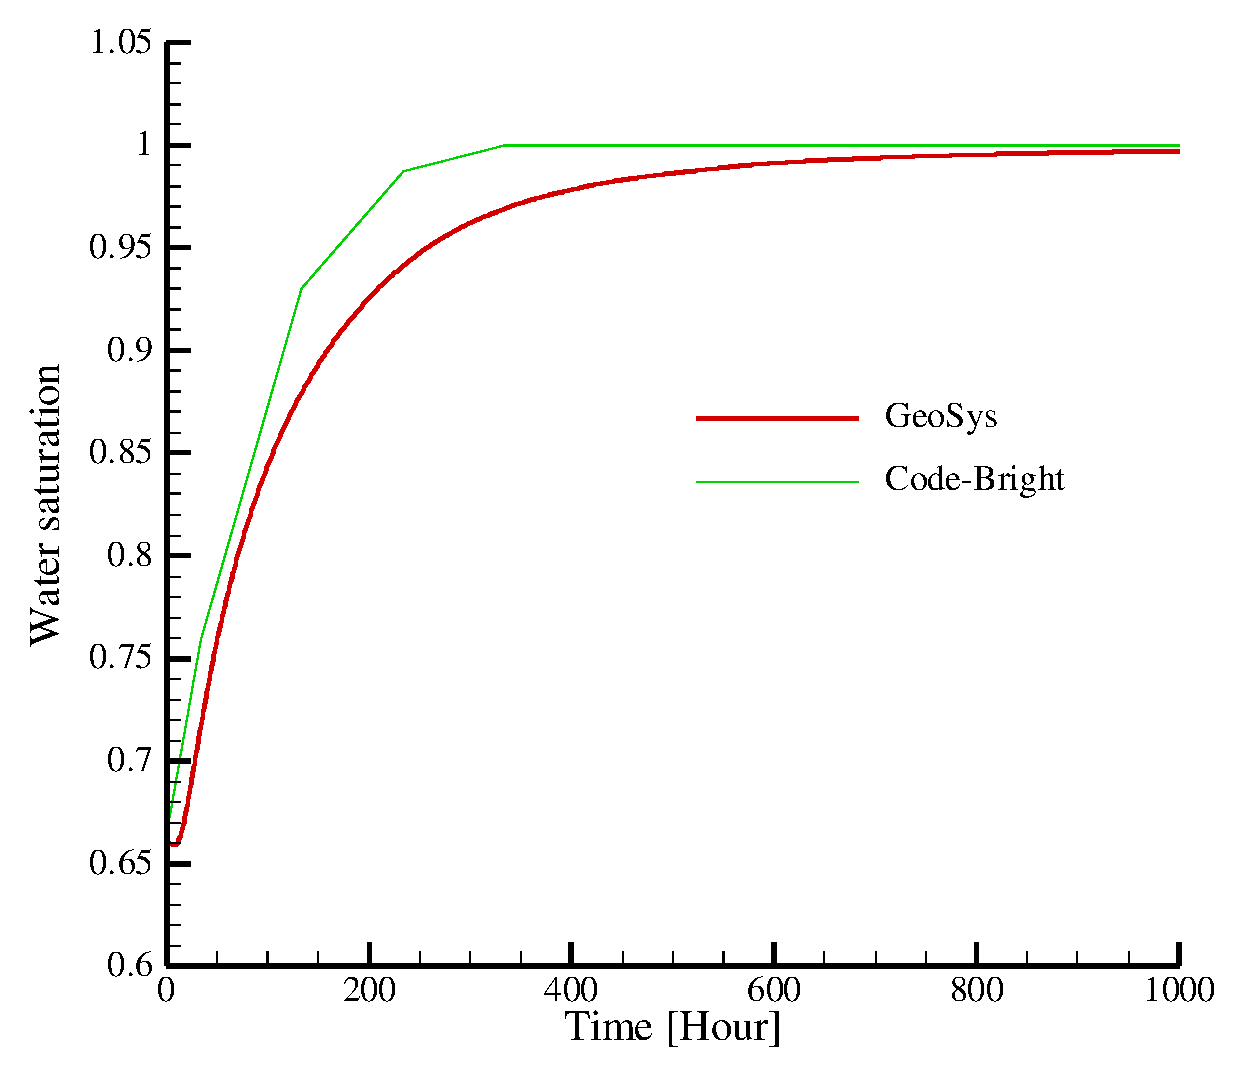
\includegraphics[width=0.7\textwidth]{chapter_14/figures/fig_14_3_25}
\end{center}
\caption{Water saturation evolution at the sample bottom.}
\label{fig:S_top}
\end{figure}
